\documentclass[12pt,a4paper,draft]{article}

\usepackage[utf8]{inputenc}
\usepackage{mathbbol}
\usepackage[bookmarks=false,colorlinks,urlcolor=blue,%
linkcolor=magenta,citecolor=red,linktocpage=true,breaklinks=true]{hyperref}
\usepackage{graphicx}
\usepackage{inconsolata}
\renewcommand*\contentsname{Indice}

\title{Jollar -- A Jolie Based Criptocurrency}
\author{Stefano Pio Zingaro}

\begin{document}

\maketitle

\begin{abstract}
Il progetto si propone di creare un sistema di scambio elettronico decentralizzato, in cui gli utenti effettuano transazioni certificate dalla rete stessa, senza il bisogno di un organo centrale garante (come ad esempio una banca). Il progetto è sviluppato seguendo i principi della programmazione orientata ai (micro)servizi, in cui la comunicazione tra i processi è implementata nel linguaggio visto a lezione: Jolie.
\end{abstract}

\tableofcontents

\section{Informazioni Logistiche}
\subsection{Formazione dei Gruppi}
%
I gruppi possono essere costituiti da un minimo di 3 a un massimo di 5 persone. 
I gruppi che intendono svolgere questo progetto, devono comunicare via email a \url{stefanopio.zingaro@unibo.it} entro il \textbf{10 Maggio 2018} la composizione del gruppo. 
L'email deve avere come oggetto \textbf{GRUPPO LSO} e contenere:
\begin{enumerate}
    \item Nome del gruppo;
    \item Una riga per ogni componente del gruppo, con cognome, nome e matricola;
    \item Un indirizzo email di riferimento a cui mandare le notifiche al gruppo, sarà poi suo incarico trasmetterle agli altri membri.
\end{enumerate}
Email di esempio con oggetto \textbf{GRUPPO LSO}

\noindent\textit{NomeGruppo}
\begin{itemize}
    \item \textit{Zingaro, Stefano, 123456}
    \item \textit{Pallino, Pinco, 234567}
    \item \textit{Banana, Joe, 345678}
\end{itemize}
\textit{Referente:} \url{stefano.zingaro@studio.unibo.it}

Chi non comunicherà la composizione del gruppo entro il \textbf{10 Maggio 2018} non potrà consegnare il progetto. 
Nel caso, chi non riuscisse a trovare un gruppo, lo comunichi il prima possibile, entro e non oltre il \textbf{7 Maggio 2018}, a \url{stefano.zingaro@studio.unibo.it} con una mail con oggetto \textbf{CERCO GRUPPO LSO}, specificando:
\begin{enumerate}
    \item Cognome, Nome, Matricola, Email;
    \item Eventuali preferenze legate a luogo e tempi di lavoro (si cercherà di costituire gruppi di persone con luoghi e tempi di lavoro compatibili)
\end{enumerate}
Email di esempio con oggetto \textbf{CERCO GRUPPO LSO} 
\begin{itemize}
    \item \textit{Zingaro, Stefano, 123456,} \url{stefano.zingaro@studio.unibo.it}
\end{itemize}
\textit{Preferisco trovarci nei pressi del dipartimento, tutti i giorno dopo pranzo.}

Le persone senza un gruppo verranno raggruppate il prima possibile \textbf{e non sarà possibile modificare i gruppi formati}.
%
\subsection{Date dell'Orale}
%

\section{Componenti del Progetto e loro Implementazione}
In generale, il sistema consiste in una rete \textit{Peer-To-Peer} (\textbf{P2P}) che utilizza \textit{Proof-of-Work} (\textbf{POW}) per registrare l'elenco delle transazioni in un archivio pubblico, detto \textbf{blockchain}. Per una migliore comprensione del fenomeno si rimanda alla lettura dell'articolo originale di Satoshi Nakamoto \href{https://bitcoin.org/bitcoin.pdf}{Bitcoin}. 
L'implementazione del progetto è, almeno in parte, ripresa da quella descritta nell'articolo, fatta eccezione per lo sviluppodella Proof-of-Work, che segue i principi della criptovaluta \href{http://primecoin.io/bin/primecoin-paper.pdf}{\textbf{Primecoin}}.

In questa sezione sono enunciate le definizioni di transazioni (contenute in un blocco) e blockchain, e se ne discute la relativa implementazione. Sono poi elencate le definizioni delle altre componenti del sistema: il meccanismo di convalida di un blocco (la Proof-of-Work); il server Timestamp per la sincronizzazione oraria; il comportamento della rete all'avvio dell'esecuzione.

\subsection{Le transazioni e la catena di blocchi: la Blockchain}
La \textbf{blockchain} è una struttura dati ordinata, una lista concatenata di blocchi contenenti transazioni. L'intera struttura della blockchain può essere conservata in un file, oppure in un database. Un \textbf{block}, o blocco, è un contenitore, una struttura dati a sua volta, che aggrega transazioni che devono essere incluse in un \textit{ledger}\footnote{Il termine ledger indica il libro mastro dei contabili, viene tradotto in italiano come registro.} pubblico e condiviso, la blockchain. 
Il blocco è composto da un \textit{header}, che contiene i \textit{metadata}, e dalla lista di transazioni che ne compongono la maggior parte della grandezza. Di seguito un esempio in Jolie di un tipo ``custom''.

\subsubsection{Implementazione}
\begin{enumerate}
    \item L'ID del blocco;
    \item Il hash del blocco precedente;
    \item Lunghezza della Proof-of-Work;
    \item Il numero primo origine (descritto più avanti);
    \item La catena di numeri primi che compone la Proof-of-Work di quel blocco;
\end{enumerate}

%
\lstinputlisting[language=Jolie]{code/block.ol}
%

\noindent In Jolie la funzione di Hash MD5 (da 128 bit) si trova già implementata nell'interfaccia \texttt{MessageDigest}.
%
\lstinputlisting[language=Jolie]{code/hash.ol}
%

\subsection{Il Server Timestamp}
Un server timestamp offre un servizio che permette di conoscere l'ora esatta all'interno della rete. Un nodo che intende effettuare le operazioni di scrittura o di validazione di un blocco deve richiedere il \textbf{timestamp} al server. Esso garantisce l'esistenza dei dati al momento della richiesta.

\subsubsection{Implementazione}
In particolare, Jolie offre, tramite l'interfaccia \texttt{time} una \texttt{operation} che restituisce i millisecondi del \textit{current unix timestamp} nel momento esatto della richiesta. Tramite una chiamata a tale servizio si può ottenere il dato necessario da includere nel blocco. Qui è riportato un esempio si chiamata a tale operation, che può essere inserita in un server che accetta richieste e le inoltra al servizio time.
%
\lstinputlisting[language=Jolie]{code/timestamp.ol}
%

\subsection{La Proof-of-Work}
La Proof-of-Work, è un algoritmo che viene utilizzato per raggiungere un accordo decentralizzato tra diversi nodi nel processo di aggiunta di un blocco specifico alla blockchain.
Tale algoritmo produce valori che vengono utilizzati per verificare che sia stata eseguita una notevole quantità di lavoro. Nell'immagine riportata qui sotto viene visualizzato un esempio di utilizzo di tecniche Proof-of-Work nel mondo delle criptovalute (in particolare quella di Ethereum ma generalizzabile a qualunque altra che usa Proof-of-Work).
Per implementare un sistema decentralizzato basato su rete P2P, abbiamo bisogno di usare un sistema di Proof-of-Work\footnote{\url{http://www.wisdom.weizmann.ac.il/~naor/PAPERS/pvp.ps}}. Questo metodo consiste nell'obbligare i nodi che vogliono scrivere un blocco a cercare un valore che sia difficile da trovare e di cui sia facile controllarne la correttezza da parte degli altri nodi che vogliono validare la scrittura.
\begin{center}
    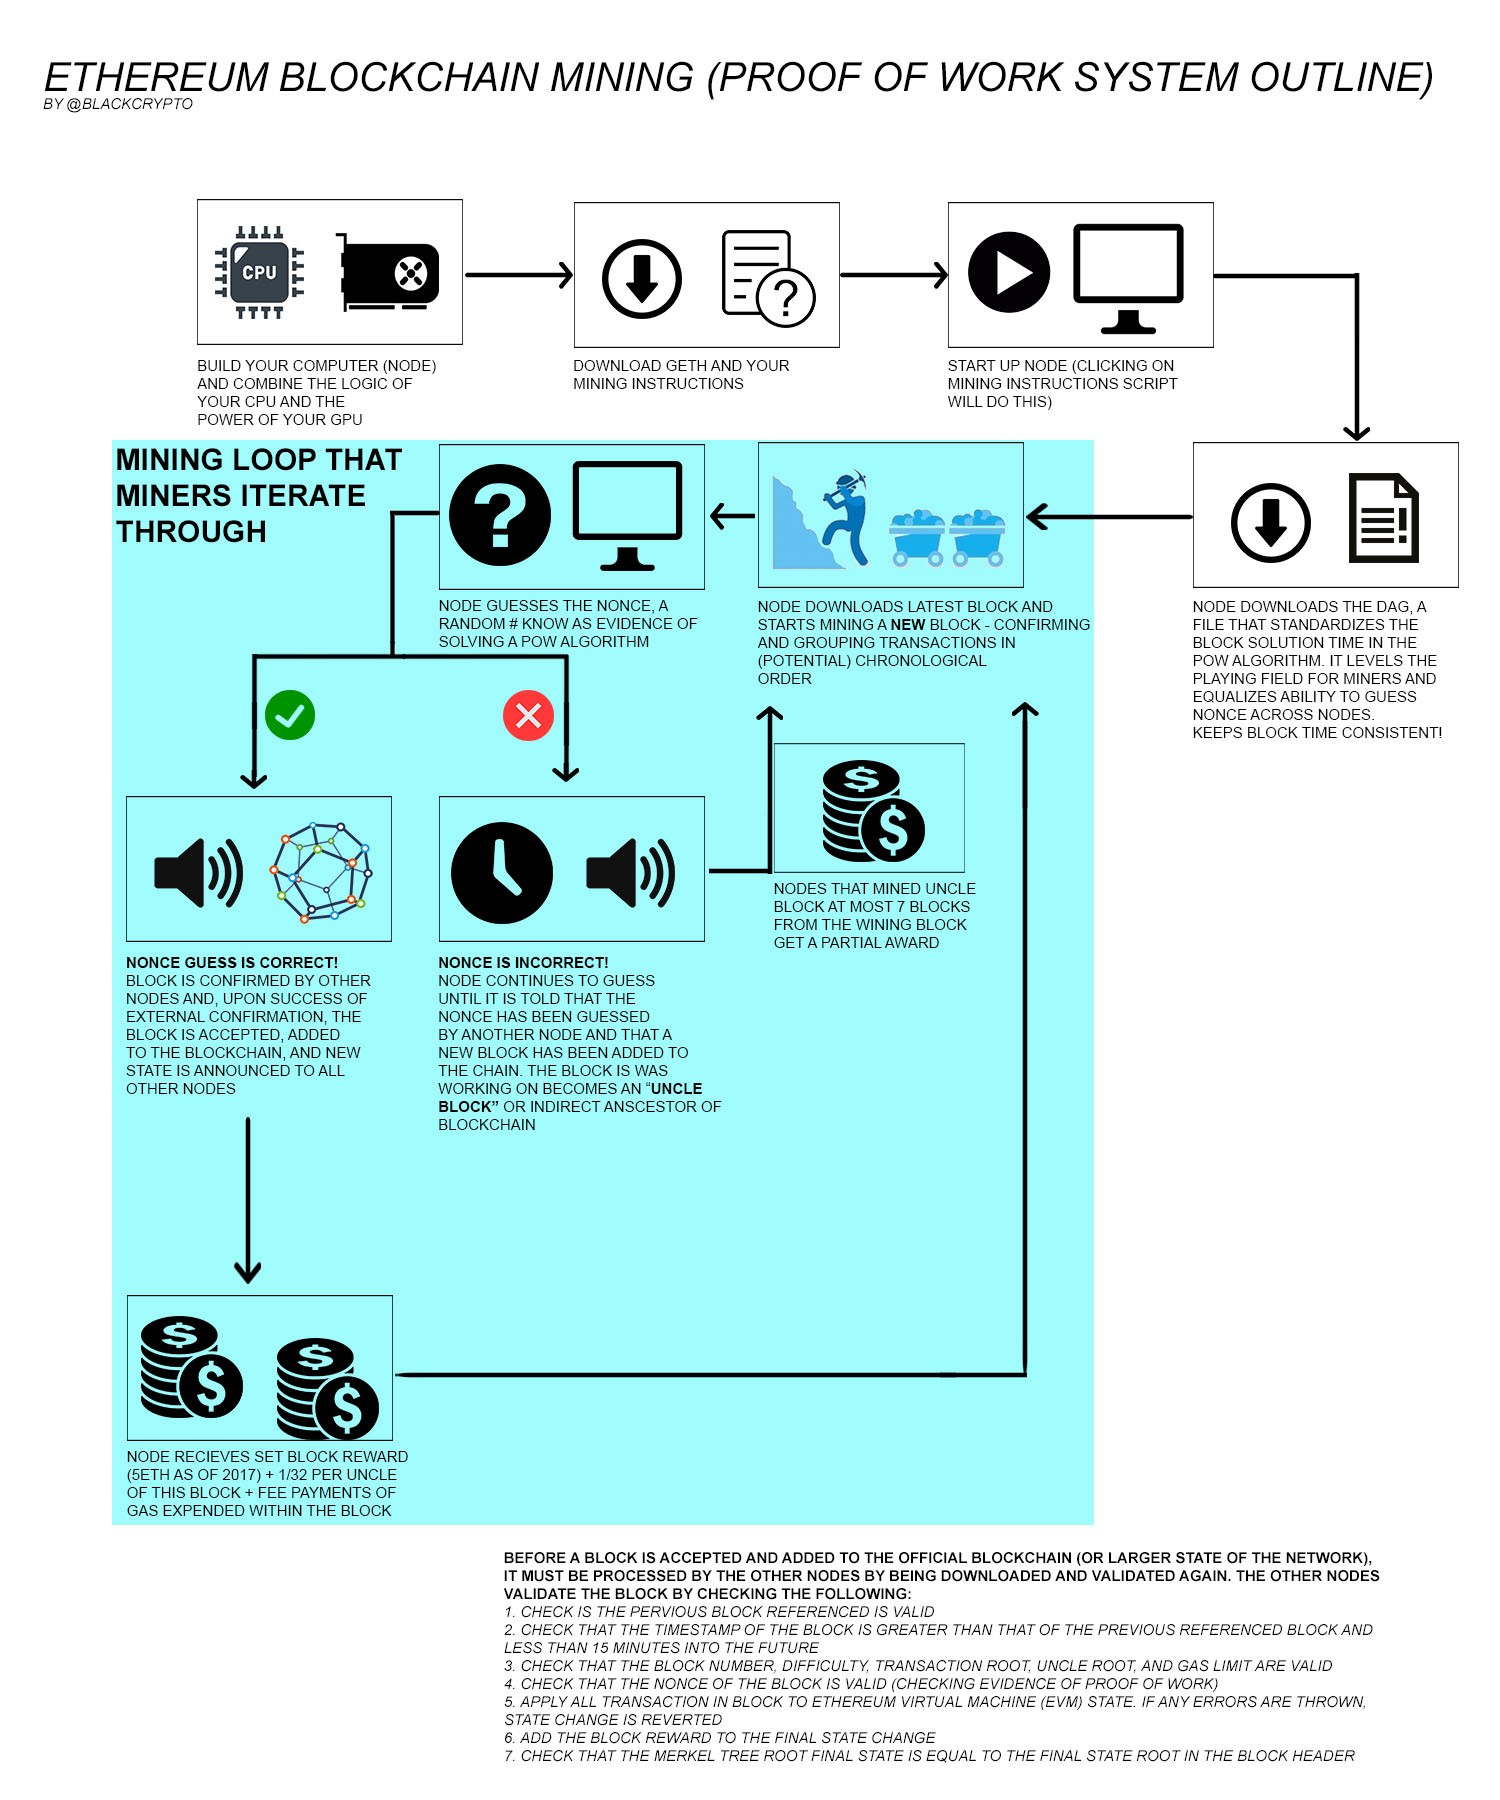
\includegraphics[width=\linewidth]{img/pow}
\end{center}

\subsubsection{Implementazione}
La Proof-of-Work scelta per produrre blocchi ed ottenere così sei Jollar in \textit{reward}\footnote{A differenza di Bitcoin, il reward in questo caso è fissato a sei ed è costante per tutta la vita della rete, un \textit{improvement} possibile è cambiare questo valore in una funzione decrescente.} è quella utilizzata dalla moneta PrimeCoin. Essa consiste nel generare delle catena di numeri primi con determinate proprietà.

\subsubsection*{Catene di Cunningham del Primo Tipo}
Una catena di Cunningham del primo tipo di lunghezza $k$ è un array di numeri primi:
\begin{center}
    $n-1,2n-1,\dots,2^{k-1}n-1$
\end{center}
Il numero $n$ è chiamato l'\textbf{origine} della catena. L'origine di una catena va va incluso nel blocco! Un esempio:
\begin{itemize}
    \item origine: $n=5$
    \item lunghezza: $k=5$
    \item catena: $2,5,11,23,47$
\end{itemize}

\subsubsection*{Catene di Cunningham del Secondo Tipo}
Una catena di Cunningham del secondo tipo di lunghezza $k$ è un array di numeri primi:
\begin{center}
    $n-1,n+1,2n-1,2m+1,\dots,\dots,2^{k-1}n-1,2^{k-1}n+1$
\end{center}
Un esempio:
\begin{itemize}
    \item origine: $n=4$
    \item lunghezza: $2k=4(k=2)$
    \item catena: $5,7,11,13$
\end{itemize}

\subsubsection*{Catene Bi-twin}
Una catena di Bi-twin di lunghezza $2k$ è una catena di $k$ numeri primi
\begin{center}
    $n-1,2n-1,\dots,2^{k-1}n-1$
\end{center}
 Un esempio:
\begin{itemize}
    \item origine: $n=5$
    \item lunghezza: $k=5$
    \item catena: $5,7,11,13$
\end{itemize}
Le catene Bi-twin posso anche essere viste come l'unione di due catene di Cunningham del primo o del secondo tipo con la stessa origine e lunghezza.
%
\subsection*{Validazione delle catene}
Il meccanismo di controllo e validazione delle Proof-of-Work inviate contenenti le catene di numeri primi prevede un test che utilizza il piccolo Teorema di Fermat (\href{http://primes.utm.edu/notes/proofs/FermatsLittleTheorem.html}{link alla dimostrazione}), esso afferma che, per $p$ primo ed $a$ intero 
\begin{center}
$a^{p-1} \equiv 1 (\bmod p)$ se $p$ non divide $a$.
\end{center}

\noindent I $p$ che soddisfano questo proprietà vengono chiamati \textit{pseudoprimi}, perché non tutti sono appunto primi. Vale però che maggiore è $p$, maggiore è la probabilità che sia primo. 

\noindent Un esempio utilizza tipicamente $a=2$ e lo eleva alla $p-1$ (prendiamo $17$ e $23$) che modulo p risulta essere uguale ad $1$:
\begin{center}
$2^{16}= 65536 \bmod 17 = 1$ \\
oppure \\
$2^{22}= 4194304 \bmod 23 = 1$
\end{center}

Ciò significa che per la primalità va controllata per ogni numero primo della catena. Inoltre la validazione controlla anche che la lunghezza della catena sia maggiore o uguale alla difficoltà (quindi il tipo di catena va incluso nel blocco!)

\subsection{La Rete Peer-To-Peer}
Una rete P2P, come ad esempio quella di \href{www.emule-project.net/home/perl/}{Emule}, è una rete i cui nodi non sono \textbf{client} o \textbf{server} fissi, ma prendono forma di entità equivalenti o ``paritarie''.
\begin{center}
    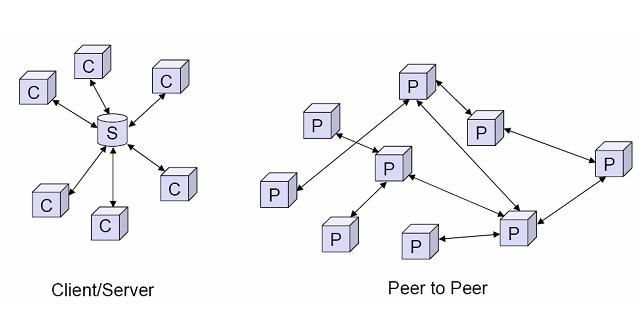
\includegraphics[width=\linewidth]{img/p2p}
\end{center}

\subsubsection{Implementazione}
L'esecuzione della rete P2P comprende i seguenti passaggi:
\begin{enumerate}
    \item Le nuove transazioni sono inviate in \textit{broadcast}\footnote{Nelle reti di calcolatori, il termine broadcast indica una modalità di instradamento per la quale un pacchetto dati inviato ad un indirizzo particolare (detto appunto di broadcast) verrà consegnato a tutti i computer collegati alla rete} a tutti i nodi che partecipano alla rete;
    \item Ogni nodo colleziona la nuove transazione in un blocco (una transazione per blocco!);
    \item Ogni nodo effettua del ``lavoro'' per provare di poter scrivere il blocco (Proof-of-Work);
    \item Quando un nodo trova una prova, invia il blocco in broadcast a tutti i nodi;
    \item I nodi accettano il nuovo blocco solo se la transazione contenuta in esso è valida e non è stata già ``spesa'';
\end{enumerate}

I nodi considerano sempre la blockchain più lunga come quella corretta. Nel caso in cui due nodi inviano versioni differenti del nuovo blocco contemporaneamente, alcuni nodi potrebbero riceverne  una versione, altri l'altra. In quel caso il nodo lavora sul blocco ricevuto temporalmente prima. Il nodo che ha lavorato su un blocco non sincronizzato se ne rende conto quando una nuova validazione viene richiesta, in questo caso egli manda in broadcast una richiesta di sincronizzazione sul blocco in questione e, una volta ricevuta risposta, aggiorna la blockchain alla versione più recente, potendo così validare il nuovo blocco ricevuto.

\subsection{Il Network Visualiser}
Il Network Visualiser è un tool amministrativo da terminale per il monitoraggio del sistema.

\subsubsection{Implementazione}
Il Network Visualizer invia richieste a tutta la rete per conoscere lo stato delle blockchain di tutti i nodi, la loro versione, le transazioni che contengono, generando le seguenti informazioni:
\begin{itemize}
    \item La data e l'ora del server timestamp al momento della richiesta.
    \item Per ogni utente/nodo: la sua chiave pubblica; le transazioni che ha effettuato divise per entrate/uscite; la versione della blockchain che utilizza e la quantità totale di Jollar che possiede.
    \item Per ogni transazione al punto precedente, ordinate in ordine cronologico, si indica la data, l'ora, e gli utenti (con le loro chiavi pubbliche) coinvolti.
    \item La blockchain più lunga presente nella rete (chiamata la versione ufficiale), con tutta la struttura dati che contiene.
\end{itemize}

\section{Specifiche di Consegna}
%
\subsection{Il Report}
%
\subsubsection{Modalità di Consegna}
%
\subsubsection{Griglia di Valutazione}
%
\subsection{La Demo}
%
\subsubsection{Modalità di Consegna}
%
\subsubsection{Griglia di Valutazione}
%
\subsection{L'Implementazione}
%
\subsubsection{Modalità di Consegna}
%
\subsubsection{Griglia di Valutazione}
%
In generale, il sistema consiste in una rete \textit{Peer-To-Peer}~(\textbf{P2P}) che utilizza tecniche di \textit{Proof-of-Work}~(\textbf{POW}) per registrare l'elenco delle transazioni in un archivio pubblico, detto \textbf{blockchain}. 
Una rete P2P, come ad esempio quella di Emule\footnote{\url{www.emule-project.net/home/perl/general.cgi?l=18}}, è una rete i cui nodi non sono \textbf{client} o \textbf{server} fissi, ma prendono forma di entità equivalenti o ``paritarie''.
%
\begin{center}
    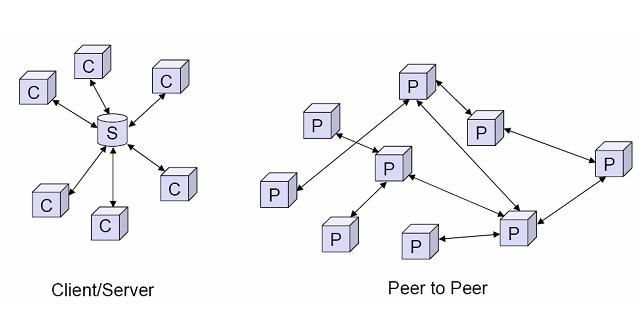
\includegraphics[width=.7\linewidth]{img/p2p}
\end{center}
%
La PoW, è un algoritmo che viene utilizzato per raggiungere un accordo decentralizzato tra diversi nodi nel processo di aggiunta di un blocco specifico alla blockchain.
Tale algoritmo produce valori che vengono utilizzati per verificare che sia stata eseguita una notevole quantità di lavoro. Nell'immagine riportata qui sotto viene visualizzato un esempio di utilizzo di tecniche POW nel mondo delle criptovalute (in particolare quella di Ethereum ma generalizzabile a qualunque altra che usa POW).
%
\begin{center}
    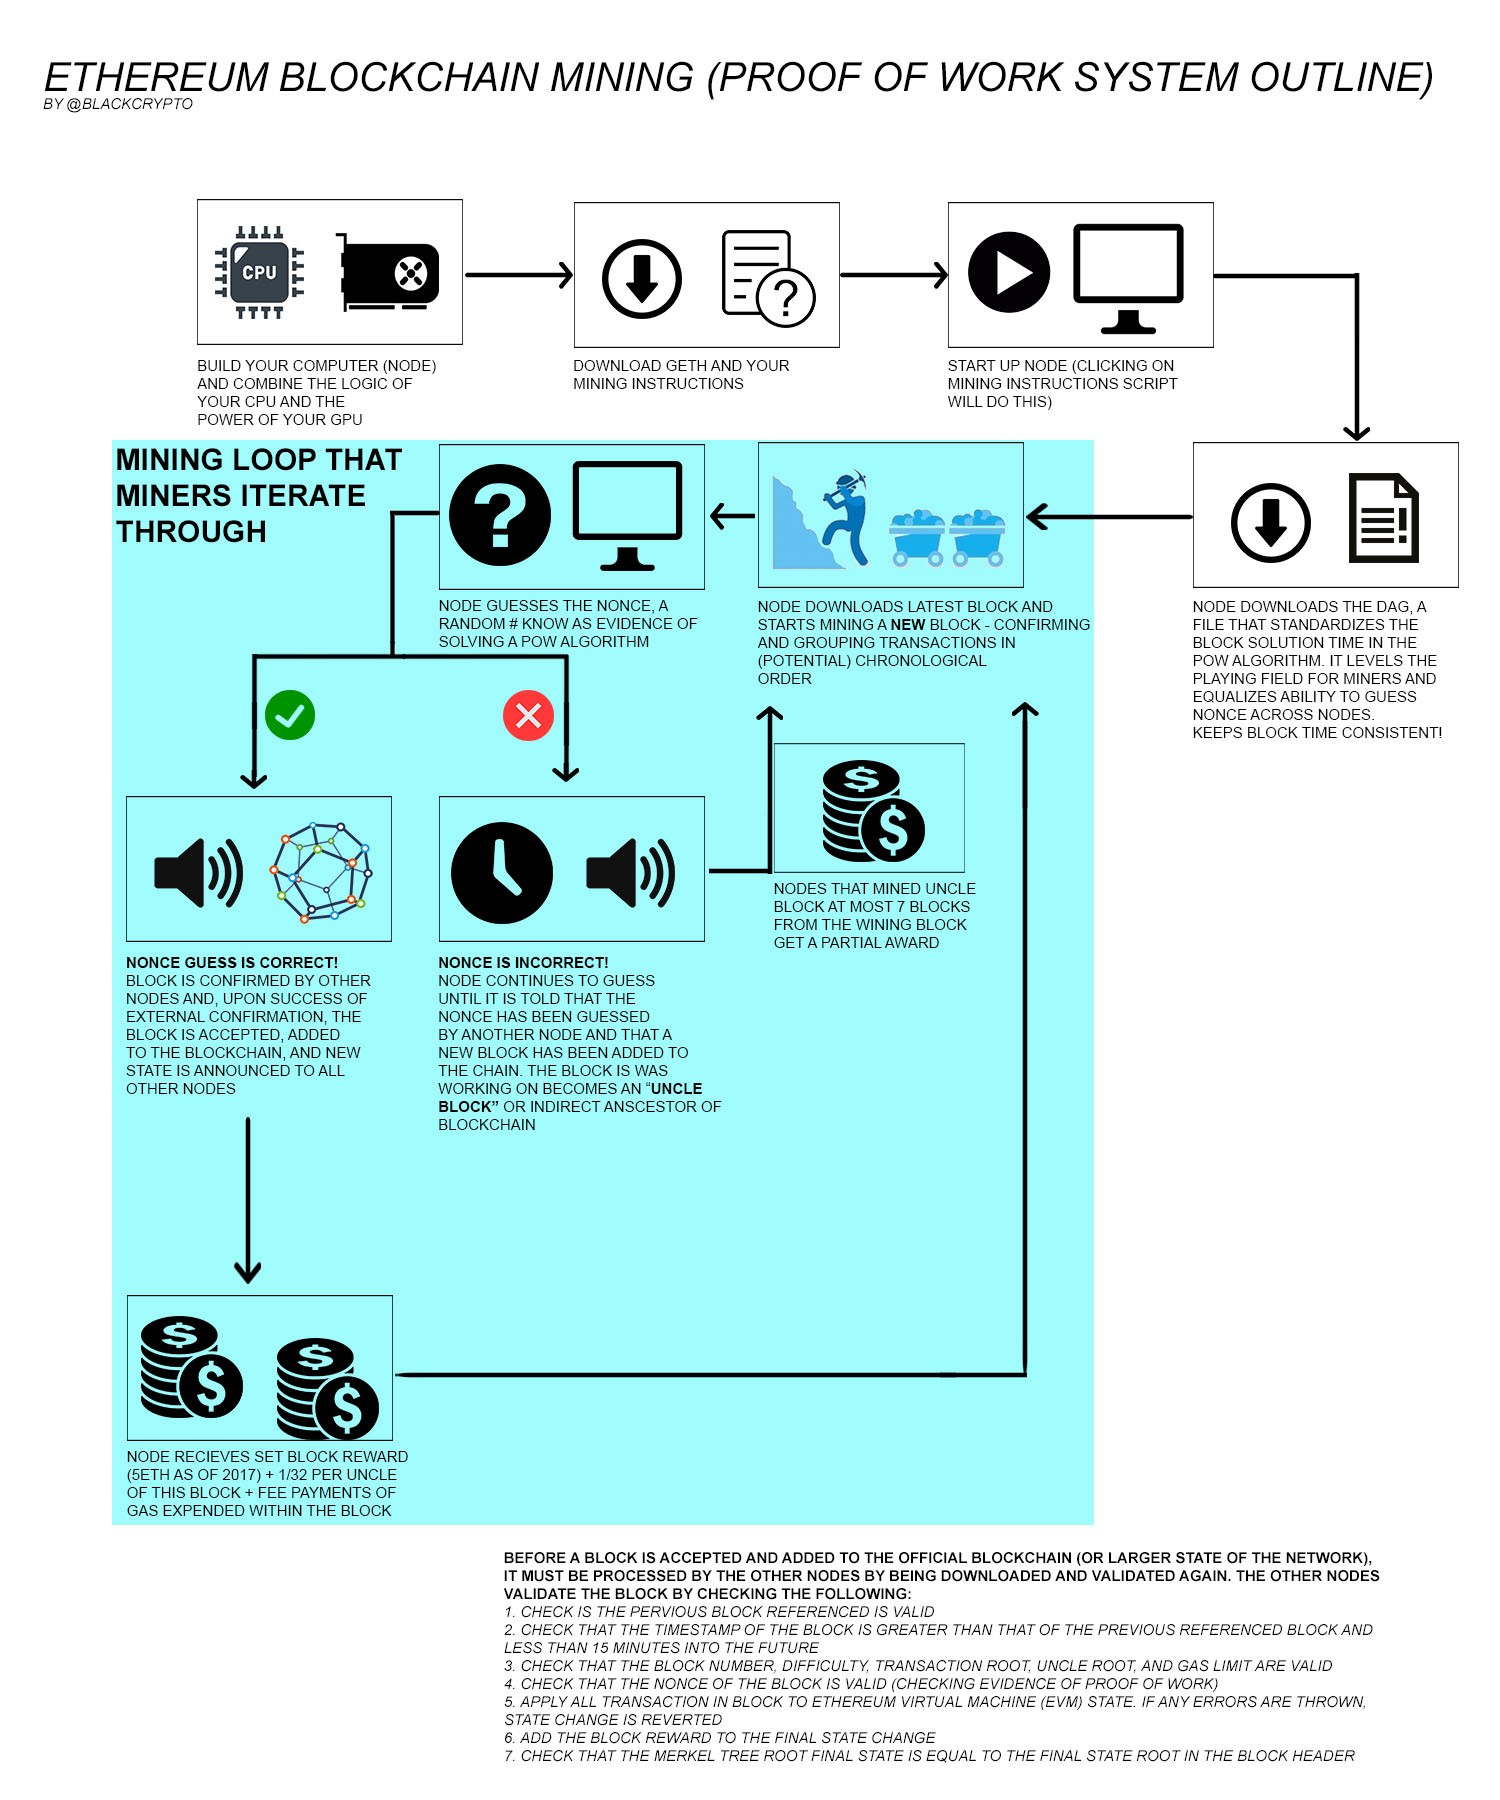
\includegraphics[width=\linewidth]{img/pow}
\end{center}
%
La \textbf{blockchain} è una struttura dati ordinata, una lista concatenata di blocchi contenenti transazioni.
L'intera struttura della blockchain può essere conservata in un file, oppure in un database.
Un \textbf{block}, o blocco, è un contenitore, una struttura dati a sua volta, che aggrega transazioni che devono essere incluse in un \textit{ledger}\footnote{termine che indica il libro mastro dei contabili, viene tradotto come registro.} pubblico e condiviso, la blockchain. 
Il blocco è composto da un \textit{header}, che contiene i \textit{metadata}, e dalla lista di transazioni che ne compongono la maggior parte della grandezza.
\subsection{Le Transazioni}
%
%
\subsection{Il Server Timestamp}
%
%
\subsection{La Proof-of-Work}
%
Per implementare un server timestamp basato su rete P2P, abbiamo bisogno di usare un sistema di proof-of-work\footnote{\url{http://www.wisdom.weizmann.ac.il/~naor/PAPERS/pvp.ps}}. Questo metodo consiste nell'obbligare i nodi che vogliono scrivere un blocco a cercare un valore che sia difficile da trovare e di cui sia facile controllarne la correttezza da parte degli altri nodi che vogliono validare la scrittura.
%
\begin{itemize}
    \item \textbf{Indice}: Un numero primo $p$ deve essere generato, una buona pratica sarebbe quella di generare un numero primo abbastanza grande, quindi si consiglia l'utilizzo di tipi \texttt{Long}. I \texttt{Long} in Java, quindi anche in Jolie, hanno un limite superiore pari a $9,223,372,036,854,775,807$. Oltre questo numero il sistema semplicemente termina di produrre prove.
    \item \textbf{Definizione}: $f_p(x) \equiv \sqrt{x} \bmod p$, cioè equivale ad estrarre tutte le radici quadrate modulo il numero primo $p$. Il dominio di $f_p$ è $\mathbb{Z}_p$.
    \item \textbf{Verifica}:  Dati $x,y$ controllare che $y^2 \equiv x \bmod p$.
\end{itemize}
%
Il meccanismo di controllo prevede solo una moltiplicazione, mentre non esiste un metodo veloce per l'estrazione delle radici modulo un numero primo, che non richieda meno di $\log{p}$ moltiplicazioni. Ne consegue che maggiore sia la lunghezza di $p$, maggiore sarà lo sforzo computazionale necessario, e quindi maggiore la differenza di tempo per valutare $f_p$ e per verificarne la correttezza.
%
\subsection{La Rete Peer-To-Peer}
%

\subsection{Il Network Visualizer}
Il Network Visualiser è un tool amministrativo da terminale per il monitoraggio del sistema.

\section{Consegna del Progetto}
Il progetto deve essere sviluppato utilizzando il linguaggio Jolie.
Non ci sono requisiti riguardo ai protocolli (\textit{protocol}) e i media (\textit{location}) utilizzati per realizzare la comunicazione tra i componenti dello Shop. 
L'obiettivo riguarda la gestione concorrente di risorse condivise. 
L'importante è dimostrare che il comportamento implementato gestisca i tipici problemi di concorrenza su risorse condivise (e.g., il tipico problema \texttt{Readers-Writers}).

\textbf{N.B.} Uno dei punti di valutazione riguarda l'uso del parallelismo nel progetto. 
Ad esempio usare execution { sequential } per prevenire scritture (e letture) parallele è una soluzione al problema considerato, ma rappresenta anche una notevole perdita in termini di concorrenza, incidendo negativamente sulla valutazione del progetto.

\subsection{Report}
Il report, scritto in word o \LaTeX, dovrà avere le seguenti caratteristiche formali:
\begin{enumerate}
    \item Dovrà avere lunghezza di quattro o cinque pagine (da 4 a 5 pagine equivalgono da 8 a 10 facciate).
    \item Dovrà essere scritta in singola colonna con font di grandezza \textbf{12pt}.
    \item Deve essere consegnato in formato PDF.
\end{enumerate}
In contenuto del report avrà discussioni in particolare sui seguenti argomenti:
\begin{itemize}
    \item la struttura del progetto (la divisione delle funzionalità tra i servizi e la loro gerarchia);
    \item le scelte più importanti fatte sul progetto e come sono state sviluppate, con esempi di codice;
    \item i problemi principali riscontrati, le alternative considerate e le soluzioni scelte;
    \item le istruzioni per eseguire il progetto e quelle per eseguire una demo di esecuzione. 
\end{itemize}
\textit{Questo punto è particolarmente importante, scrivete le specifiche come se tutto il programma dovesse essere eseguito da una persona che non sa nulla del progetto, dopo almeno 2 anni dal momenti in cui è stato scritto}.

\subsubsection{Demo}
La demo conterrà almeno 5 nodi della rete, 1 server timestamp, 1 Network Visualizer per osservare l'esecuzione dei comandi.
La sequenza di esecuzione suggerita è la seguente:
\begin{enumerate}
    \item avvio del Server Timestamp;
    \item avvio del Network Visualizer;
    \item avvio in cascata dei nodi.
\end{enumerate}
A questo indirizzo è disponibile un canovaccio, in markdown, con la struttura del report. 
Pandoc\footnote{\url{http://cs.unibo.it/~sgiallor/teaching/project/current/report_template.md}} permette di creare PDF da markdown. 
È possibile scrivere il report nel formato preferito (.doc, .tex), l'importante è che il PDF generato rispetti la struttura del modello.
%
\subsection{Gruppi}
%


\subsection{Consegna e Date}
%
Lo sviluppo del progetto avviene col supporto di \textit{Git}\footnote{\url{http://rogerdudler.github.io/git-guide/index.it.html}}, così come la consegna del progetto.
I gruppi devono creare un repository su GitLab\footnote{\url{http://gitlab.com}} seguendo la procedura descritta sotto.
%
\newline\noindent
Creazione del gruppo:
\begin{itemize}
    \item ogni membro del gruppo crea un account su GitLab;
    \item il referente del gruppo:
    \begin{itemize}
        \item crea un progetto cliccando sul \textbf{+} in alto a destra nella schermata principale di GitLab, inserendo il nome ``LabSO\_NomeGruppo'' (dove NomeGruppo è il nome registrato in precedenza del gruppo) e cliccando su \textbf{Create Project};
        \item una volta che il progetto è stato creato, aggiunge membri al progetto andando su \textbf{Settings} $>$ \textbf{Members};
        \item aggiunge ogni membro del gruppo come \textbf{Developer}, cercandoli in base allo username registrato su GitLab;
        \item aggiunge l'utente ``@stefanopiozingaro'' come \textbf{Reporter}.
    \end{itemize}
\end{itemize}
%
Al momento della consegna, il repository dovrà contenere i sorgenti del progetto e la relazione, nominata \textbf{REPORT\_LSO.pdf}. 
È possibile inserire un file di nome \textbf{README} che riporti istruzioni su come lanciare gli eseguibili.
Per effettuare la consegna, il \textbf{referente del gruppo} crea un \textbf{Tag} del progetto. 
Per creare un \textbf{Tag} del progetto:
\begin{enumerate}
    \item nella pagina di progetto su GitLab, cliccare sulle voci \textbf{Repository} $>$ \textbf{Tags} $>$ \textbf{New Tag}; 
    \item digitare come \textbf{Tag Name} il nome \textbf{Consegna} e lasciare gli altri campi vuoti;
    \item cliccare su \textbf{Create Tag} per eseguire la creazione del \textbf{Tag} di consegna.
\end{enumerate}
%
Una volta creato il Tag, inviare una email di notifica di consegna con soggetto \textbf{CONSEGNA LSO - NOME GRUPPO} a \url{stefanopio.zingaro@unibo.it}.
Il report va anche consegnato in forma cartacea nella casella del prof. Sangiorgi (piano terra del Dipartimento di Informatica, a fianco del suo ufficio). Ci sono due date di consegna disponibili:
\begin{itemize}
    \item le 23.59(UTC+1) di Lunedí 2 Luglio 2018;
    \item le 23.59(UTC+1) di Lunedí 17 Settembre 2018.
\end{itemize}
\textbf{Come data di consegna, farà fede la data di creazione del Tag su GitLab.}
In seguito alle consegne, verranno fissate data e ora della discussione del progetto compatibilmente coi tempi di correzione. 
La data di discussione verrà notificata ai gruppi tramite la mail di riferimento.

\subsubsection{Valutazione}
Il progetto verrà valutato mediante una discussione di gruppo, con tutti i componenti del gruppo presenti. 
Non è possibile per i componenti di un gruppo effettuare la discussione in incontri separati. 
Al termine della discussione, ad ogni singolo componente verrà assegnato un voto in base all'effettivo contributo dimostrato nel lavoro di progetto. 
La valutazione del progetto è indipendente dal numero di persone che compongono il gruppo.

\subsubsection{Note Importanti}
\begin{itemize}
    \item non si accettano email o richieste di eccezioni sui progetti con motivazioni legate a esigenze di laurearsi o di non voler pagare le tasse per un altro anno.
    \item chi copia o fa copiare, anche solo parte del progetto, si vedrà invalidare completamente il progetto senza possibilità di appello. Dovrà quindi rifare un nuovo progetto l'anno successivo. Durante la correzione verrà utilizzato un tool per la ricerca di codice copiato.
\end{itemize}

\subsection{Domande sul Progetto e Ricevimento}
Per le domande sul progetto si consiglia di usare il newsgroup del corso. 
Risposte corrette alle domande dei colleghi sul newsgroup verranno valutate positivamente in sede di esame. 
È possibile chiedere informazioni o un ricevimento via email, specificando la motivazione della richiesta, a \url{stefanopio.zingaro@unibo.it}.

\end{document}